\documentclass[11pt]{article}

\usepackage{fontspec}
\usepackage[vietnamese]{babel}

\usepackage{graphicx}
\usepackage{amsmath, amssymb, amsfonts, bm}
\usepackage{xcolor}
\usepackage{hyperref}
\usepackage{pifont}
\newcommand{\xmark}{\ding{55}}
\newcommand{\cmark}{\ding{51}}
\usepackage{array}
\usepackage{float}

\hypersetup{
    colorlinks=true,
    linkcolor=blue,
    filecolor=magenta,
    urlcolor=red,
    pdftitle={Overleaf Example},
    pdfpagemode=FullScreen,
}

\setmainfont{Times New Roman}
\setsansfont{Arial}
\setmonofont{Courier New}


% Page layout
\setlength{\topmargin}{-.5in}
\setlength{\textheight}{9.25in}
\setlength{\oddsidemargin}{0in}
\setlength{\textwidth}{6.8in}

% Title formatting
\usepackage{titling}
\setlength{\droptitle}{-10em}
\pretitle{%
    \begin{center}
    \LARGE\bfseries\textcolor{green}
    \end{center}
}
\posttitle{%
    \begin{center}
    \LARGE\bfseries\textcolor{cyan}
    \end{center}
}
\title{{Module Project}\\[0.5em]\textcolor{cyan}{RAG (Retrieval-Augmented Generation) sử dụng Streamlit}}
\author{Đinh Nhật Thành}
\date{}
\renewcommand{\maketitle}{}

% Fancy header/footer
\usepackage{fancyhdr}
\pagestyle{fancy}
\fancyhf{}
\renewcommand{\footrulewidth}{0.4pt}
\lhead{\bfseries AI VIETNAM}
\rhead{\bfseries aivietnam.edu.vn}
\fancyfoot[C]{\thepage}

% Section format (không đánh số section)
\usepackage{titlesec}
\titleformat{\section}
{\normalfont\Large\bfseries}
{}{0em}{}

% Listings (code block)
\usepackage{listings}
\definecolor{codegreen}{rgb}{0,0.6,0}
\definecolor{codegray}{rgb}{0.5,0.5,0.5}
\definecolor{codepurple}{rgb}{0.58,0,0.82}
\definecolor{backcolour}{rgb}{0.95,0.95,0.92}
\lstdefinestyle{mystyle}{
    backgroundcolor=\color{backcolour},
    commentstyle=\color{codegreen},
    keywordstyle=\color{magenta},
    numberstyle=\tiny\color{codegray},
    stringstyle=\color{codepurple},
    basicstyle=\ttfamily\footnotesize,
    breaklines=true,
    captionpos=b,
    keepspaces=true,
    numbers=left,
    numbersep=5pt,
    tabsize=2,
    showspaces=false,
    showstringspaces=false,
    showtabs=false
}
\lstset{style=mystyle}

% Colored boxes
\usepackage[many]{tcolorbox}
\definecolor{sub}{HTML}{cde4ff}
\newtcolorbox{boxC}{
    colback = sub,
    boxrule = 0pt
}

% For math proofs or custom counters (tuỳ chọn nếu cần)
\usepackage{lipsum}
\newcounter{mycounter}
\newcommand\showmycounter{\stepcounter{mycounter}\themycounter}
\newcommand\showlips{\stepcounter{mycounter}\lipsum[\value{mycounter}]}

% Others
\usepackage{booktabs}
\usepackage{subcaption}
\usepackage{framed}
\usepackage{tikz}


%%%%%%%%%%%%%%%%%%%%%%%%%%%%%%%%%%%%%%%%%%%%%%%%%%%%%%%%%%%%%%%%%%%%%%%%%%%%%
%%%%%%%%%%%%%%%%%%%%%%%%%%%%%%%%%%%%%%%%%%%%%%%%%%%%%%%%%%%%%%%%%%%%%%%%%%%%%
%%%%%%%%%%%%%%%%%%%%%%%%%%%%%%%%%%%%%%%%%%%%%%%%%%%%%%%%%%%%%%%%%%%%%%%%%%%%%
\begin{document}
\maketitle

\begin{titlepage}
    \centering
    \vspace*{\fill}

    {\Huge \textbf{\thetitle} \par}
    \vspace{2em}

    {\Large \textbf{\theauthor} \par}
    \vspace{1em}

    {\large \today \par}

    \vspace*{\fill}
    \thispagestyle{fancy}
\end{titlepage}

\newpage
\tableofcontents
\thispagestyle{fancy}


%1%%%%%%%%%%%%%%%%%%%%%%%%%%%%%%%%%%%%%%%%%%%%%%%%%%%%%%%%%%%%%%%%%%%%%%%%%%%%%%%%%%%%%%%%%%%%%%%%%%%%%%%%%%%%%%%%%%%%%%%%%%%%%%%%%%%%%%%%%%%%%%%%%%%%%%%%%%%%%%%%%%%%%%%%%%%%%%%%%%%%%%%
\newpage

\renewcommand{\thesubsection}{\arabic{subsection}}
\newpage

\subsection{Giải thích thuật ngữ}

Để giúp người đọc dễ dàng nắm bắt các khái niệm trong báo cáo, dưới đây là giải thích chi tiết một số thuật ngữ quan trọng:

\begin{itemize}
    \item \textbf{Parse (Phân tích cú pháp):}
    \begin{boxC}
        Trong lập trình và xử lý dữ liệu, "parse" là quá trình \textbf{chuyển đổi một dạng dữ liệu} (thường là một chuỗi văn bản, số, hoặc bất kỳ loại dữ liệu thô nào) \textbf{thành một cấu trúc dữ liệu có ý nghĩa}.
        \begin{itemize}
            \item Ví dụ: Khi một chương trình "parse" một chuỗi văn bản, nó sẽ phân tích và chia nhỏ chuỗi đó thành các phần nhỏ hơn, có ý nghĩa (gọi là "tokens") dựa trên một tập hợp các quy tắc (ngữ pháp). Mục đích là để máy tính có thể hiểu và làm việc với dữ liệu đó dễ dàng hơn.
            \item Minh họa: Hãy xem xét biểu thức toán học "4+10". Đối với máy tính, đây chỉ là các ký tự riêng lẻ '4', '+', '1', '0'. Để thực hiện phép tính, máy tính phải "parse" biểu thức này. Một chương trình phân tích cú pháp sẽ nhận diện '+' là phép cộng, và từ đó biết rằng các ký tự đứng trước và sau nó là các chữ số biểu thị hai số cần cộng. Nó sẽ tạo ra một cấu trúc mới để biểu diễn thông tin này một cách tốt hơn cho phần tiếp theo của chương trình, ví dụ như chuyển "4" thành số nhị phân 100 và "10" thành 1010, và biểu thức "4+10" thành một dạng dễ hiểu hơn cho máy tính như: `ADD 100 1010`.
        \end{itemize}
    \end{boxC}

    \item \textbf{Protocol (Giao thức):}
    \begin{boxC}
        Là một tập hợp các quy tắc, định dạng và quy trình chuẩn mực \textbf{quy định cách dữ liệu được truyền tải và nhận giữa các thiết bị hoặc chương trình} trong một mạng. Giao thức đảm bảo rằng các bên tham gia có thể giao tiếp một cách hiệu quả và hiểu được thông điệp của nhau.
    \end{boxC}

    \item \textbf{Synchronous (Đồng bộ) và Asynchronous (Bất đồng bộ):}
    \begin{boxC}
        Đây là hai khái niệm thường gây nhầm lẫn vì chúng liên quan đến \textbf{thời gian thực hiện đồng thời}, không nhất thiết là luồng thực thi trong lập trình. Tóm lại, các tác vụ bất đồng bộ không bắt đầu và kết thúc cùng một lúc.

        \begin{itemize}
            \item \textbf{Lập trình Đồng bộ (Synchronous Programming - "Từng việc một"):} Trong ngữ cảnh lập trình, \textbf{việc bắt đầu của một tác vụ được đồng bộ hóa với việc hoàn thành của tác vụ trước đó}. Các tác vụ xảy ra theo một trình tự cứng nhắc và phối hợp.
            \begin{itemize}
                \item Các hoạt động thực thi từng tác vụ một, mỗi tác vụ phải hoàn thành hoàn toàn trước khi tác vụ tiếp theo có thể bắt đầu.
            \end{itemize}
            \item \textbf{Lập trình Bất đồng bộ (Asynchronous Programming - "Đa tác vụ đồng thời"):} Trong ngữ cảnh lập trình, \textbf{việc bắt đầu của một tác vụ không được đồng bộ hóa với việc hoàn thành của một tác vụ khác}. Chúng có thể chồng lấn trong quá trình thực thi.
            \begin{itemize}
                \item Các hoạt động trong lập trình bất đồng bộ \textbf{cho phép một chương trình tiếp tục thực thi 1 hoặc nhiều tác vụ trong khi chờ đợi một tác vụ khác hoàn thành} (thường là các hoạt động tốn nhiều thời gian) mà không chặn luồng chính.
                \item Lưu ý rằng khi chạy bất đồng bộ trên một luồng đơn (single thread), đó chỉ là việc luồng đơn chuyển đổi nhanh chóng giữa các tác vụ khác nhau, tạo ra ảo giác về tính song song.
                \item Lợi ích của lập trình bất đồng bộ thường được nhận thấy rõ rệt nhất trong Giao diện người dùng (User Interface - UI), nó giúp UI không bị "đóng băng" khi một hoạt động nặng đang chạy ngầm.
            \end{itemize}
        \end{itemize}
    \end{boxC}
\end{itemize}


\section{Tóm tắt ý chính}
Hệ thống được xây dựng nhằm hỗ trợ người dùng truy vấn thông tin từ tài liệu PDF bằng cách sử dụng mô hình ngôn ngữ lớn (LLM)
kết hợp với cơ sở dữ liệu vector. Người dùng upload tài liệu PDF lên giao diện web được xây dựng bằng Streamlit,
hệ thống sẽ tự động chia nhỏ văn bản, mã hoá thành vector, và sử dụng RAG để sinh ra câu trả lời theo truy vấn.

\section{Hệ thống RAG sử dụng Streamlit}

\subsection*{Kiến trúc hệ thống}

Hệ thống bao gồm các thành phần chính sau:

\begin{enumerate}
    \item Giao diện người dùng bằng \textbf{Streamlit}.
    \item Phân tích và trích xuất văn bản từ file PDF.
    \item Chia nhỏ nội dung thành các đoạn (chunk) bằng \texttt{SemanticChunker}.
    \item Mã hóa và lưu trữ các đoạn văn bản dưới dạng vector sử dụng \texttt{HuggingFaceEmbeddings} và cơ sở dữ liệu \texttt{Chroma}.
    \item Truy hồi thông tin liên quan dựa trên câu hỏi người dùng.
    \item Tạo prompt tùy chỉnh và gửi đến mô hình LLM để sinh câu trả lời.
\end{enumerate}

\begin{figure}[H]
    \centering
    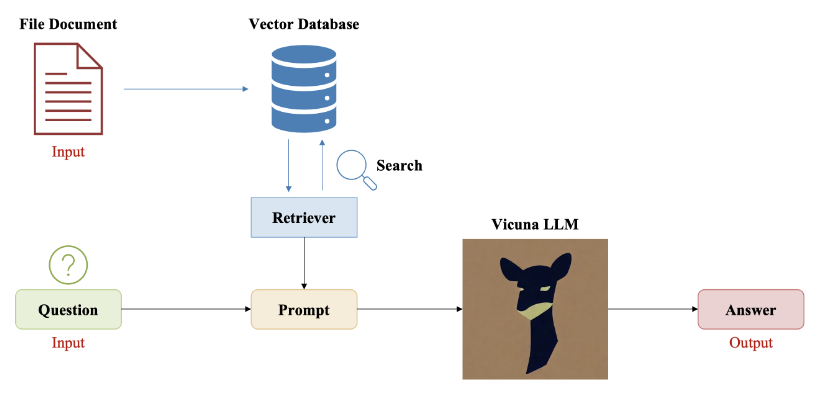
\includegraphics[width=0.85\textwidth]{architecture.png}
    \caption{Kiến trúc tổng quan của hệ thống RAG}
\end{figure}

\section{Giới thiệu tổng quan về mô hình RAG}
\subsection{Giải thích RAG và các thành phần cốt lõi}

\subsection{Vấn đề tồn tại khi xây dựng mô hình RAG và giải pháp cơ bản của Native RAG, giải pháp LangChain đưa ra}

\subsubsection*{Giải pháp cơ bản của Native RAG}

\subsubsection*{Giải pháp LangChain đưa ra}

\section{Giới thiệu LangChain và vai trò của nó trong xây dựng RAG}

\subsection{LangChain là gì?}

\subsection{Vai trò của LangChain trong việc xây dựng RAG}
\subsection{Giải thích căn bản về các syntax của LangChain}

Trong LangChain, các \textbf{Runnable} là những khối xây dựng cơ bản, mỗi Runnable đại diện cho một tác vụ hoặc hoạt động đơn lẻ. Về bản chất, một Runnable là một đối tượng Python được thiết kế để tối ưu hóa hàm của bạn bằng cách sử dụng tính song song.

\subsubsection*{Khái niệm chính về Runnables trong LangChain}
\begin{itemize}
    \item \textbf{Tính mô đun (Modularity):}
    \begin{boxC}
        Mỗi \texttt{Runnable} là một khối xây dựng đại diện cho một nhiệm vụ hoặc thao tác đơn lẻ. Các nhiệm vụ này có thể bao gồm chạy một LLM (Mô hình Ngôn ngữ Lớn), xử lý dữ liệu hoặc xâu chuỗi nhiều hoạt động lại với nhau.
    \end{boxC}

    \item \textbf{Tính kết hợp (Composability):}
    \begin{boxC}
        Nhiều \texttt{Runnable} có thể được liên kết với nhau để hình thành một chuỗi (pipeline). Điều này cho phép xây dựng các quy trình làm việc phức tạp từ các thành phần nhỏ hơn, có thể tái sử dụng.
    \end{boxC}

    \item \textbf{Tính tái sử dụng (Reusability):}
    \begin{boxC}
        Các \texttt{Runnable} có thể được tái sử dụng trong các quy trình làm việc khác nhau.
    \end{boxC}

    \item \textbf{Thực thi bất đồng bộ (Asynchronous Execution):}
    \begin{boxC}
        Các \texttt{Runnable} có khả năng thực hiện các tác vụ một cách song song, tăng hiệu suất cho các ứng dụng.
    \end{boxC}
\end{itemize}

\subsubsection*{Các thành phần API cốt lõi}

\begin{enumerate}
    \item \textbf{Runnable: Lớp cơ sở (Object)}
    \begin{boxC}
        \texttt{Runnable} là lớp cơ sở cho tất cả các thành phần có thể thực thi trong LangChain. Bạn có thể kế thừa từ lớp này để tạo các thao tác tùy chỉnh của mình.
        \begin{lstlisting}[language=Python, caption=Ví dụ về Runnable cơ bản]
from langchain.schema.runnable import Runnable

class MyRunnable(Runnable):
    def invoke(self, input):
        return input.upper()

# Tạo một thể hiện của MyRunnable
runnable = MyRunnable()

# Kiểm tra với một input mẫu
result = runnable.invoke("hello world")
print(result)  # Output: HELLO WORLD

# Thử một ví dụ khác
result = runnable.invoke("LangChain is awesome")
print(result)  # Output: LANGCHAIN IS AWESOME
        \end{lstlisting}
    \end{boxC}

    \item \textbf{RunnableMap:}
    \begin{boxC}
        Tương tự như hàm \texttt{map()} trong Python, \texttt{RunnableMap} thực thi nhiều \texttt{Runnable} bên trong nó một cách song song và tổng hợp kết quả của chúng. Điều này hữu ích khi bạn muốn áp dụng nhiều hàm độc lập cho một chuỗi đầu vào và nhận các kết quả khác nhau cho từng hàm.
        \begin{lstlisting}[language=Python, caption=Ví dụ về RunnableMap]
from langchain.schema.runnable import RunnableMap

runnable_map = RunnableMap({
    "uppercase": lambda x: x.upper(),
    "reverse": lambda x: x[::-1],
})

result = runnable_map.invoke("langchain")
# Output: {'uppercase': 'LANGCHAIN', 'reverse': 'niahcnagL'}
        \end{lstlisting}
    \end{boxC}

    \item \textbf{RunnableSequence:}
    \begin{boxC}
        \texttt{RunnableSequence} áp dụng từng \texttt{Runnable} một cách tuần tự vào đầu vào. Đơn giản hơn \texttt{RunnableMap}, đầu vào được xử lý tuyến tính qua từng \texttt{Runnable}.
        \begin{lstlisting}[language=Python, caption=Ví dụ về RunnableSequence]
from langchain.schema.runnable import RunnableSequence

runnable_sequence = RunnableSequence([
    lambda x: x.lower(),
    lambda x: x[::-1],
])

result = runnable_sequence.invoke("LangChain")
# Output: 'niahcnag'
        \end{lstlisting}
    \end{boxC}

    \item \textbf{RunnableLambda:}
    \begin{boxC}
        \texttt{RunnableLambda} là \texttt{Runnable} đơn giản nhất, về cơ bản là định nghĩa một hàm lambda làm \texttt{Runnable}. Nó áp dụng một hàm duy nhất cho chuỗi đầu vào.
        \begin{lstlisting}[language=Python, caption=Ví dụ về RunnableLambda]
from langchain.schema.runnable import RunnableLambda

uppercase_runnable = RunnableLambda(lambda x: x.upper())
result = uppercase_runnable.invoke("langchain")
# Output: 'LANGCHAIN'
        \end{lstlisting}
    \end{boxC}
\end{enumerate}

\subsubsection*{Ví dụ: Quy trình làm việc đầu cuối (End-to-End Workflow)}
\begin{boxC}
    \textbf{Bài toán:} Xử lý phản hồi của khách hàng, phân loại cảm xúc và tóm tắt nó.
    \begin{enumerate}
        \item Đầu tiên mình cần tạo 1 hàm dể phân loại cảm xúc (nếu "good" thì là Positive, ngược lại là Negative) bằng cách sử dụng \texttt{RunnableLambda}.
        \item Bước tiếp theo là truy xuất ngữ cảnh, sau đó cung cấp hướng dẫn và ngữ cảnh cho LLM bằng cách sử dụng \texttt{PromptTemplate}. Điều này nghe có vẻ tuần tự, vì vậy ta sử dụng \texttt{RunnableSequence}.
        \item Bây giờ, chúng ta muốn kết hợp cả bước 1 và 2 để nhận được hai đầu ra riêng biệt: một cho cảm xúc và một cho bản tóm tắt của mô hình. Điều này phù hợp với \texttt{RunnableMap}.
    \end{enumerate}
    \begin{lstlisting}[language=Python, caption=Ví dụ về quy trình làm việc kết hợp các Runnable]
from langchain.prompts import PromptTemplate
from langchain.llms import OpenAI
from langchain.schema.runnable import Runnable, RunnableSequence, RunnableMap, RunnableLambda

# Định nghĩa các Runnables riêng lẻ
sentiment_analysis_runnable = RunnableLambda(lambda text: "Positive" if "good" in text.lower() else "Negative")

# Sử dụng OpenAI làm LLM ví dụ (cần cài đặt và cấu hình khóa API)
llm = OpenAI(openai_api_key="YOUR_OPENAI_API_KEY")

summarization_runnable = PromptTemplate(input_variables=["text"], template="Tóm tắt đoạn văn này: {text}") | llm # | đại diện cho RunnableSequence

# Kết hợp các Runnables thành một chuỗi (pipeline)
pipeline = RunnableMap({
    "sentiment": sentiment_analysis_runnable,
    "summary": summarization_runnable
})

# Gọi pipeline
feedback = "Chất lượng sản phẩm rất tốt và vượt quá mong đợi."
result = pipeline.invoke(feedback)

print(result)
# Output (có thể khác tùy thuộc vào LLM):
# {
#    "sentiment": "Positive",
#    "summary": "Chất lượng sản phẩm xuất sắc."
# }
    \end{lstlisting}
\end{boxC}

\subsubsection*{LangChain Expression Language (LCEL)}
\begin{boxC}
    \textbf{LangChain Expression Language (LCEL)} là một cú pháp được tạo ra để giúp chạy các chuỗi (chains) một cách tối ưu, dù là đồng bộ (song song) hay bất đồng bộ (không song song), bằng cách kết hợp các \texttt{Runnable} với nhau.
    LCEL rất phù hợp cho các chuỗi đơn giản (ví dụ: prompt + llm + parser). Tuy nhiên, LangGraph được khuyến nghị để mở rộng thêm khi bạn xây dựng các chuỗi phức tạp hơn (ví dụ: có phân nhánh, vòng lặp, nhiều tác nhân, v.v.). Lưu ý rằng LCEL vẫn có thể được sử dụng trong LangGraph.
\end{boxC}


\subsection{Giải pháp của LangChain cho từng vấn đề tồn tại của RAG}

\section{Demo kết quả mô hình RAG cơ bản}
\subsection*{Quy trình thực hiện}

\subsection*{Ví dụ Code Snippet (Minh họa)}
\subsection*{Kết quả minh họa}

\section{Cải Thiện Mô hình RAG}

\subsection{Prompting có cấu trúc (Structured Prompting)}

\subsection{Các kiểu Prompt khác nhau}
\subsection{Cải tiến tốc độ truy vấn sử dụng FAISS}

\subsubsection*{Lợi ích khi sử dụng FAISS:}

\subsubsection*{Cách tích hợp FAISS với LangChain:}

\section{Tổng kết}

\section{Kết Thúc}

\end{document}